\chapter{Embedded system security}

Embedded systems are distinct from other type of systems due to their varying nature ranging from programmable logic controllers (PLC), to larger systems, such as servers or routers. \cite{fysarakis2014embedded}. An usual embedded device conducts a specific task, and possibly demands networking capabilities. Working with embedded is typically with a limited set of resources, and it demands careful design when a multitude of features are needed, but the underlying systems have limited computing power. Maintaining and upgrading devices to meet the continuous need of security updates. Even services such as SSH have had history of vulnerabilities, which prove that upgradability is a fundamental base of a secure system \cite{secopsolutionHistorySecOps}. I argue that the security aspect of embedded devices could be improved significantly with the use of declarative systems.

Embedded devices demand precision and security, as their function may be very critical for variety of safety reasons, e.g in automotive industry or healthcare applications. \cite{turab2019secure} \cite{fysarakis2014embedded}. Reliability is a defining requirement for number of embedded applications; a pacemaker that doesn't function all the time reliably is completely useless. % tuohon kerro jotain declaratiivisista

As embedded is a broad field, in this thesis devices are limited to those which can run Linux kernel and provide the most basic networking capabilities. These cover architectures i686, x86\_64, arm64 supported by NixOS. PLCs and microcontrollers are outside of scope as NixOS needs a functional Linux kernel and a specific architecture to work. 

Information security perspectives using a policy modeling standard, CIA-triad is discussed, and NixOS is reflected with the use of the triads axes.

\section{Common embedded pitfalls}

Common issues regarding embedded devices are their lack of updates, weak data integrity, and the multitude of features \cite{kemmerer2003cybersecurity} \cite{fysarakis2014embedded}. For example, a toy teddy bear may have a audio recorder, data transfer capabilities and ability to geolocate itself. These kind of devices may lack firmware or software updates, and the data-transfer may be insecure.

A solution for secure data transfer would be TLS-encrypted messaging between clients. This could be achieved e.g with MQTT-protocol, but configuring certificates is extra effort. Multitude of features is a definite security problem, as the user may not be aware of them at all times. In an increasing global world, importing embedded devices from unreliable sources can prove to be a security issue. The household items may or may not adhere to latest security compliance. \cite{fysarakis2014embedded}

Attack surface of embedded systems in general range from physical access to network and geolocation problems. One way of manipulating a device, apart from directly gaining access to the operating system, are side channel attacks. Analysing the power or electromagnetic properties of device input/output can be used to determine critical aspects of a device, e.g key lengths or algorithms of security measures. Attack surface may used to gain access, or performing denial of service attacks. Geolocating is both a privacy and security issue, as location data may be used to trace identities of device users, which can lead to e.g blackmailing, physical intrusion or other means. \cite{fysarakis2014embedded}

Embedded systems have problems regarding monitoring and system administration. It's very different to have home automation system with less than 20 nodes, than to have public transport embedded fleet in a big city with 2000 nodes. As the number of devices grow, so does the challenge of monitoring and administrative tasks. Home automation has usually one person dedicated to the task; the home owner. The hypothetical setup with 2000 devices has an exponential growth of problems. Monitoring should be trivial to automatize (e.g by using tools like Prometheus), but administrative tasks are harder to automatize, due to tasks being potentially very challenging even for dedicated system administrators.


\section{NixOS as an embedded solution} \label{nixosassolution}

Declarative systems have advantages over imperative systems in reliability and safety aspects due to two things:

\begin{enumerate}

\item rollout and rollback are equally trivial tasks
\item desired configuration can be tested in a sandbox environment
  
\end{enumerate}

The first item makes it more accessible to manage a rollout strategy, as the rollout/rollback can be done multiple times or executed completely in a replicated sandbox environment, as stated in item 2. Simpler and more straight forward practical steps give space to more eloquent strategical planning. \cite{kandoi2021operating}.

NixOS provides a way to keep systems updated in relatively simple manner. Updates can be centralised, or local, if the device doesn't have enough processing power to conduct the updates in a suitable time frame. NixOS is limited to specific set of processor architectures, and cannot handle minimal embedded devices, and a similar system for smaller devices would be a suitable candidate for further study. As the NixOS configuration may be published partially or completely as open-source, the user could study what kind of features are enabled for a specific system in a consumer product.

Updatability is possible with many different platforms, but it's a problem when updating is a sole duty of a consumer, who may or may not have the adequate knowledge how or why they should update their systems. Easily updatable solutions can be in many forms, but the focal point of this thesis is a architecture with specifically NixOS.

Nix is a double edged sword for system administration tasks. On the other hand, it has a steep learning curve, but on the other hand it can make tasks that could be very challenging with traditional systems, trivial. In a well built Nix ecosystem security actions such as updating or modifying user or kernel space can be used to enhance security and in such system, any changes could easily be replicated to multiple devices, without the need for manual intervention. 

Some other clear disadvantages for NixOS in embedded use is the fact that a purely functional, declarative system inherently must use disk space more than it's imperative counterparts. In the worst case scenario, if one derivation of a system takes up 1Gb of space, when making changes, the resulting system will need 2Gbs of space. The worst case scenario rarely occurs, but due to Nix's indestructive nature, this formula of disk space demands has to be considered in an embedded setting. \cite{dolstra2007purely}

\section{Imperative and declarative systems from CIA-triad approach}

CIA-triad can be used as a tool to show conflicts between different points of information security interests. It consists of three meters: confidentiality, integrity and availability as seen in the figure \ref{ciatriad}. Confidentiality can be seen as superset of privacy. Confidential data is classified with technologies such as data encryption and user privileges. Integrity means that the data has not been tampered with, and remains untouched by unauthorised parties while it's in transit or stored e.g in a server. A way of providing integrity is checking hashes of downloaded files. Availability is a user viewpoint to the accessibility of the system. When confidentiality and integrity are pushed to the extreme, availability aspect suffers, e.g when a service enforces multi-factor authentication. \cite{pender2019parkerian}

Systems with an imperative package manager are more accessible than declarative systems as learning a new programming language with esoteric paradigm can pose extra effort. Configuring a whole Nix system demands a thorough knowledge of Nix language, and that definitely hinders the ease of access to a Nix system from a system administrator standpoint. With NixOS, an easy extent of confidentiality can be achieved via planting sufficient configuration files during device setup.

Atomic systems such as Nix have great benefits towards integrity. As the "nix store", where every installation is located is read-only, it's impossible for attackers to modify the store. That's not the case, where user with root privileges can arbitrarily modify installed programs and files.
\begin{figure}
    \centering
    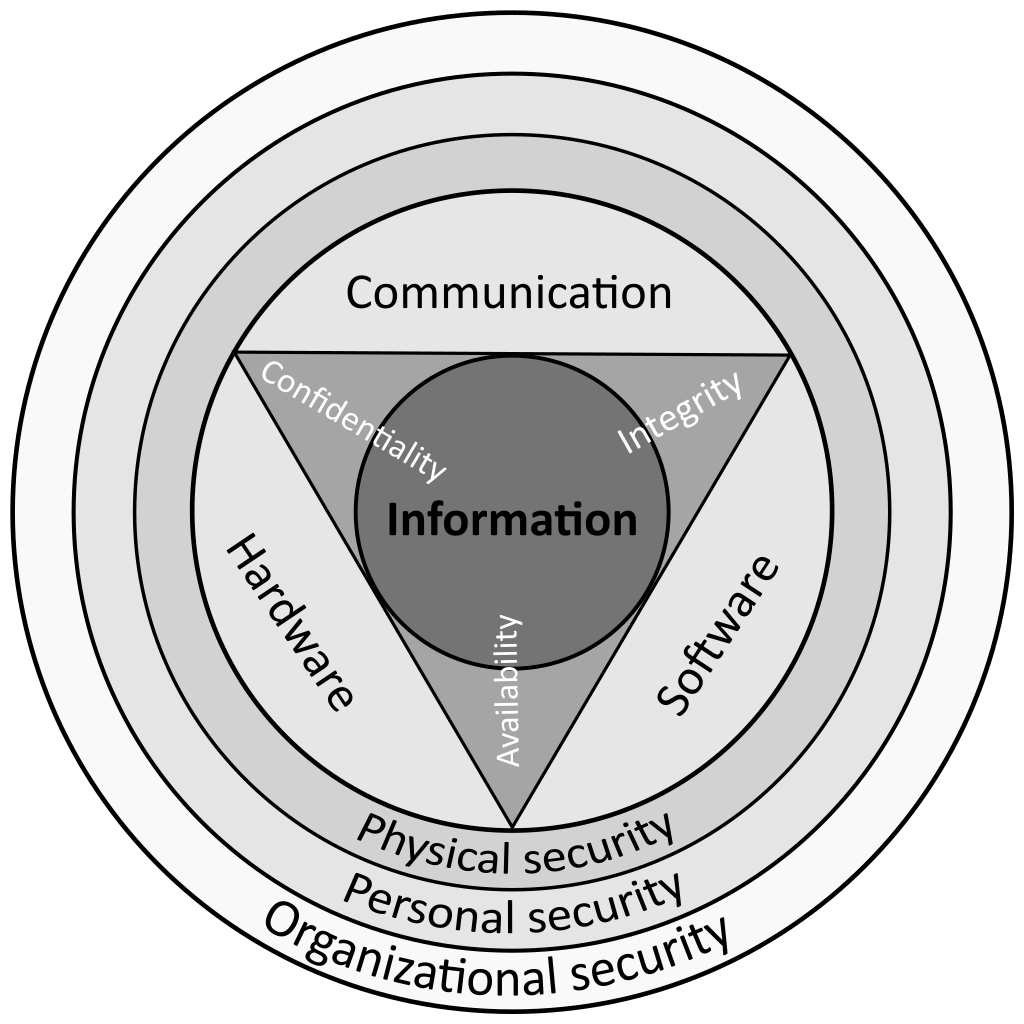
\includegraphics[scale=0.2]{latex/kuvat/ciatriad.png}
    \caption{The CIA-triad, a way to demonstrate conflicting security measures \cite{hughes2013quantitative}. (https://en.wikipedia.org/wiki/Information_security#/media/File:CIAJMK1209-en.svg)}
    \label{ciatriad}
\end{figure}
\subsection{Security by obscurity}

Currently, NixOS is quite rare in both server and desktop usage as shown in figure \ref{timeline}. Combined with the unusual file system and the usage of user-environments, some malware that rely on the usual locations of installed programs may fail \cite{nixosSecurityNixOS}.

\subsection{Multi-user installations}
The requirement for root access nearly always widen the potential attack surface. NixOS provides a way for multiple users installing their programs through the use of user environments, hence mitigating the need for root access. This both lessens the availability aspect, as well as mitigates the programs root access. When file changes are made in user-specific scope, a thin layer of isolation is achieved. \cite{nixosNixOSManual}

\subsection{Data integrity}
Data integrity is achieved both by installed programs residing in the read-only nix store, but also them having been checked against SHA256 checksums. Moreover, the core installation resources for NixOS are GPG-signed by an administrative Nix team. \cite{nixosSecurityNixOS}